\documentclass[letterpaper,12pt,twoside=false,DIV=11]{scrartcl}

%----------------------CONFIG---------------------------
%math packages
\usepackage{amsmath,amssymb,amsthm,units,unitsdef}
\usepackage{wasysym}  % astro symbols

%bibliography style and citation style, bibstyles to use: plainnat, abbrvnat, unsrtnat, named, chicago
%otherwise numerical citationstyle will be used
%\usepackage[authoryear,round]{natbib}

\usepackage{longtable,tabularx,tabulary,multirow,lscape}
\usepackage[font={sl},format=plain,labelfont=bf]{caption}

% colors
\usepackage{color,colortbl}
\usepackage[dvipsnames]{xcolor}
\definecolor{darkblue}{HTML}{00354C}

\usepackage{booktabs}
%\usepackage{showkeys} % shows the labels above the references for

%easier development
\usepackage{ifpdf}

\ifpdf
    \usepackage[pdftex]{graphicx}
    \usepackage[]{pdfpages} %for including full pdf pages
    \usepackage[pdftex,
        bookmarks,
        bookmarksopen=true,
        bookmarksnumbered=true,
        pdfauthor={Reto Trappitsch},
        pdftitle={On the origin of elements in the Milky Way - Homework},
        colorlinks,
        linkcolor=darkblue,
        citecolor=darkblue,
        filecolor=black,
        urlcolor=darkblue,
        anchorcolor=black,
        menucolor=black,
        breaklinks=true,
        pageanchor=true, %for jumping to a page
        plainpages=false,
        pdfpagelabels=true]{hyperref}
    \pdfcompresslevel=9
    \pdfoutput=1
    \DeclareGraphicsExtensions{.pdf,.png,.jpg,.jpeg}
\else
    \usepackage{graphicx}
\fi
\usepackage{rotating} % rotate figures
\usepackage{subcaption}
\usepackage{wrapfig}


\usepackage{fancyhdr}
\pagestyle{fancy}
%\addtolength{\headwidth}{\marginparsep} %these change header-rule width
%\addtolength{\headwidth}{\marginparwidth}
\lhead{}
\chead{\small\scshape On the Origin of Elements in the Milky Way} 
\rhead{} 
\lfoot{} 
\cfoot{\thepage} 
\rfoot{} 
\renewcommand{\headrulewidth}{.3pt} 
\renewcommand{\footrulewidth}{.3pt}

% Redefine author as topic
\newcommand{\topic}{\author}

%
%Redefining sections as problems
%
\makeatletter
\newenvironment{problem}{\@startsection
    {section}
    {1}
    {-.2em}
    {-3.5ex plus -1ex minus -.2ex}
    {2.3ex plus .2ex}
    {
        \pagebreak[3] % forces pagebreak when space is small; use \eject for better results
        \noindent\sffamily\bfseries Problem
    }
}
{
    %\vspace{1ex}\begin{center} \rule{0.3\linewidth}{.3pt}\end{center}}
    \begin{center}\large\bfseries\ldots\ldots\ldots\end{center}
}
\makeatother

% set enumerate to use letters
\renewcommand{\theenumi}{\alph{enumi}}

% newcommands
%============
% my short cuts
\providecommand{\e}[1]{\ensuremath{\times 10^{#1}}}
\providecommand{\ex}[1]{\ensuremath{^{#1}}}
\providecommand{\dex}[1]{\ensuremath{\delta^{#1}}}
\newcommand{\nean}{$^{22}$Ne($\alpha$,n)$^{25}$Mg}

% textnormal
\newcommand{\tn}{\textnormal}
% textregistered
\newcommand{\tr}{$^\tn{\textregistered}$}


%-------------------DOCUMENT---------------------------

\begin{document}


\title{Homework \#5 -- Solution}
\topic{Mass Spectrometry, Stardust}
\date{}

\maketitle
\thispagestyle{fancy}

\begin{problem}{Time-of-Flight Mass Analyzer (20\%)}

For an ion of mass $m$, we can set the electric energy equal to the kinetic energy and solve the equation for time.
\begin{align}
    E_\mathrm{el} &= E_\mathrm{kin}\\
    qU &= \frac{m}{2}v^2\\
    v &= \frac{d}{t}\\
    \Rightarrow qU &= \frac{m}{2} \frac{d^2}{t^2}\\
    \Rightarrow t &= \sqrt{\frac{md^2}{2qU}}\\
    t &= \frac{d}{\sqrt{2U}} \sqrt{\frac{m}{q}} \qed
\end{align}
The proportionality factor contains the flight distance $d$ and the voltage of extraction $U$. These are both instrument constants.

\end{problem}

\begin{problem}{Delta-Values (20\%)}
\begin{enumerate}
    \item   \begin{align}
                \delta^{46}\mathrm{Ti}_{48} &= \left(\frac{0.2}{\frac{204}{1820}} - 1\right) \times 1000 \permil\\
                &= 784\permil
            \end{align}
    \item This would mean that there is no \ex{46}Ti in the sample, or an infinite amount of \ex{48}Ti.
\end{enumerate}
\end{problem}

\begin{problem}{Solar System Contamination (20\%)}

First, let us calculate the zironium isotope ratios as given for the last thermal pulse of the Lugaro et al. (2018) models. To do so we need to look up the solar ratios, which are as following:
\begin{align}
    \frac{^{92}\mathrm{Zr}}{^{94}\mathrm{Zr}} &= 0.987 \equiv {^{92}}r_{\odot}\\
    \frac{^{96}\mathrm{Zr}}{^{94}\mathrm{Zr}} &= 0.161 \equiv {^{96}}r_{\odot}
\end{align}
We now reverse the $\delta$-values for the $s$-component to determine real ratios. This gives us:
\begin{align}
    \frac{^{92}\mathrm{Zr}}{^{94}\mathrm{Zr}} &= 0.782 \equiv {^{92}}r_{\star}\\
    \frac{^{96}\mathrm{Zr}}{^{94}\mathrm{Zr}} &= 0.010 \equiv {^{96}}r_{\star}
\end{align}
Now we can calculate mixing for each axis of the plot as:
\begin{equation}
    r_\mathrm{mix} = cr_\odot + (1-c)r_\star.
\end{equation}
Here, $c$ is the fraction of contamination and goes from 0 (no contamination) to 1 (no star). We can easily calculate both axes for various amounts of contamination and transfer all these values back to $\delta$-values. Plotting this result gives us the following figure:
\begin{center}
    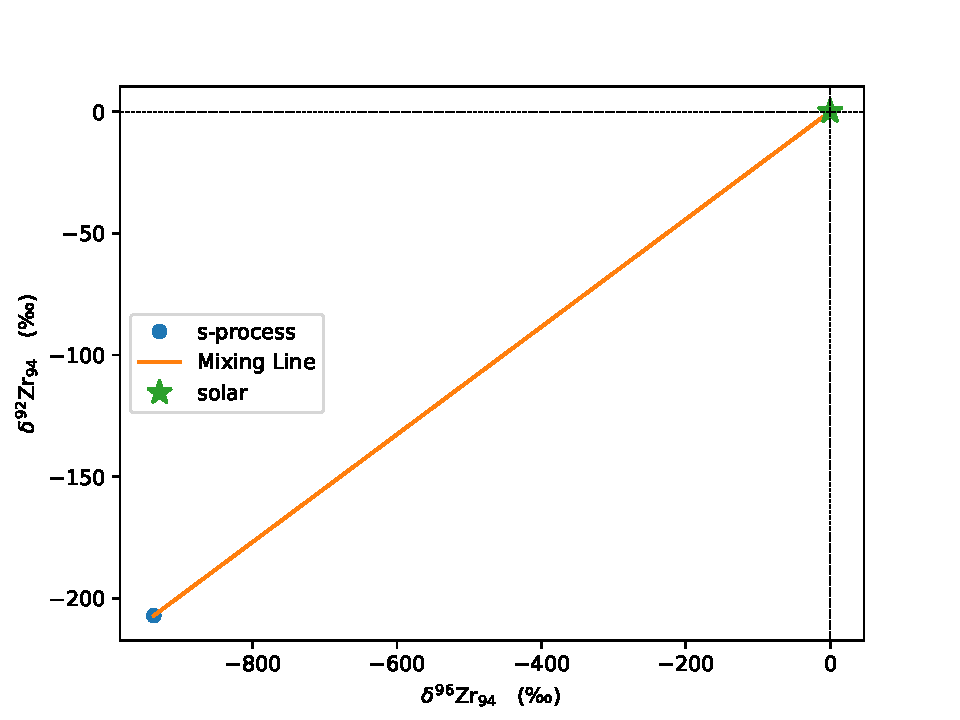
\includegraphics[width=0.75\textwidth]{mixing_line}
\end{center}


\end{problem}

\begin{problem}{Number of Atoms per Presolar Grain (20\%)}
\begin{enumerate}
    \item First we can calculate the mass of the grain $m$ as
    \begin{equation}
        m = \rho V = \rho \frac{4}{3} r^{3} \pi.
    \end{equation}
    Here, $\rho$ is the density of SiC and $r$ is the radius of the grain in question. The molecular mass of SiC is around $M = 40$\,g\,mol$^{-1}$. We can then calculate the number of moles in this grain as $\nicefrac{m}{M}$. Finally, multiplying this by Avogadro's constant, we get the number of SiC molecules in the grain:
    \begin{equation}
        n_\mathrm{SiC} = \frac{4}{3}\frac{r^3 \pi \rho}{M} N_A = 2.02\times 10^{11}.
    \end{equation}
    \item The only difficult part of this exercise is the fact that the concentration of iron is given in parts per million (ppm) by weight, however, we want to determine the number of atoms. We can do this by multiplying with the molecular masses of SiC versus iron as following:
    \begin{equation}
        n_\mathrm{Fe} = \frac{10^{-6}M_\mathrm{SiC}}{M_\mathrm{Fe}} n_\mathrm{SiC} = 1.45\times10^{6}
    \end{equation}
\end{enumerate}
\end{problem}

\begin{problem}{Solar System SiC? (20\%)}
In order for SiC to condense from a nebula, carbon must be more abundant than oxygen. In the solar nebula, however, we know that oxygen was more abundant than carbon, see, e.g., Figure~1.6 in the lecture notes. This means that SiC is not expected to condense, which explains why all SiC found in meteorites is of presolar origin. 
\end{problem}

\end{document}
